\chapter{Planning}

This chapter is about how we planned our project. The purpose of this chapter is to explain how our team is organized, who we are, why we do this project and how do it.

\section{Overall project plan}

\subsection{Project name}
XOXOmail

\subsection{Project sponsor}

The customer for this project is Thales Norway AS. Thales is a leading international electronics and systems group, focusing on defense, aerospace and security markets worldwide. The cutting edge technology in use at Thales offers capabilities unmatched in Europe for the development and deployment of mission-critical information systems proven in the field. The group’s civil and military business areas develop in parallel and share a common base of technologies to serve a single objective: the security of people, property and nations.
\newline
\newline
After Thales’ 50 years of industrial activity in Norway it is now one of Norway’s largest industrial centers of expertise for mission-critical IT and telecommunications solutions and one of the principal supplies of military communication systems to the Norwegian Armed Forces. [1]
\newline
\newline
See table \ref{tab:customer} at page \pageref{tab:customer}
\begin{table}
\begin{tabular}{l|l|l|l}
\textbf{Name} & \textbf{Office} & \textbf{Phone nr} & \textbf{E-mail} \\ \hline \hline
Sølve Conradi Olsen & Thales Norway & 907 80 179 & solve.olsen@thalesgroup.com \\ hline
Christian Tellefsen & Thales Norway & 959 98 765 & christian.tellefsen@thalesgroup.com \\ hline
Stig Bjørlykke & Thales Norway & 982 29 806 & stig.bjorlykke@thalesgroup.com
\end{tabular}
\caption{The customer representatives} \label{tab:customer}
\end{table}

\subsection{Involved Parties}

In this project there are only three involved parties: a) the customer b) the project team and c) the advisor. The customer, Thales, described in the section above was represented by Christian Tellefsen and Stig Bjørlykke. The project team consists of 6 students from the Department of Computer and Information Science (IDI) at the Norwegian University of Science and Technology (NTNU).The advisor was Mohsen Anvaari who was assigned to our team to guide and help us during the project period.
\newline
\newline
See table \ref{tab:projectgroup} at page \pageref{tab:projectgroup}
\begin{table}
\begin{tabularx}{\linewidth}{>{\setlength\hsize{.52\hsize}}X|>{\setlength\hsize{0.5\hsize}}X|>{\setlength\hsize{.3\hsize}}X|>{\setlength\hsize{.5\hsize}}X}
\textbf{Name} & \textbf{Address} & \textbf{Phone nr} & \textbf{E-mail} \\ \hline \hline
Ida Thoresen & Klæbuveien 143, 7031 & 936 68 688 & idakatt@stud.ntnu.no\\ \hline
Kristin Tønnesen & Lars Onsagersvei 12, 7030 & 986 28 958 & kristonn@stud.ntnu.no \\ \hline
Lars Høysæter & Innherredsveien 2a, 7014 & 900 31 814 & larssmor@stud.ntnu.no\\ \hline
Nicklas Utgaard & Odd Brochmanns veg 47, 7030 & 976 87 790 & nicklau@stud.ntnu.no\\ \hline
Magnus Ulstein & & 472 31 418 & magnuul@stud.ntnu.no\\ \hline
Aleksander Sjåfjell & Odd Brochmanns veg 60, 7030 & 456 01 212 & aleksasj@stud.ntnu.no
\end{tabularx}
\caption{The project group} \label{tab:projectgroup}
\end{table}

See table \ref{tab:advisor} at page \pageref{tab:advisor}
\begin{table}
\begin{tabular}{l|l|l|l}
\textbf{Name} & \textbf{Work} & \textbf{Phone nr} & \textbf{E-mail} \\ \hline \hline
Mohsen Anvaari & PhD-stud. NTNU & 405 70 403 & mohsena@idi.ntnu.no
\end{tabular}
\caption{Our advisor} \label{tab:advisor}
\end{table}

\subsection{Background for the project}

This project was given to us as an assignment in the course TDT4290 Customer Driven Project. Since the society is constantly changing, the technology must follow along with the enormous changes we see today. Because of these changes Thales found that they needed a handheld android version of their existing XOmail system. This new handheld system would help the users of XOmail so that they could also use it in the field and not only at the office. When able to use this mailing system not only in contact with a computer, the regular working day of Thales customers would be a lot easier, especially since their primary customer is the Norwegian military.

\subsection{Measurement of project effects}

Thales has proposed the following effects:
\begin{itemize}
\item{}Test user interface for message-based communication on a handheld device.
\item{}Make a prototype that can give inspiration for further product development and be used as a demonstration internally and to customers.
\end{itemize}

\newpage
\subsection{General terms}

\subsubsection{Technical Limitations}

\paragraph{Android}
Android is a quite new platform and none of us have been doing much programming in it before starting on this project. So learning how Android works and finding technical tools that Android supports is going to be a time consuming task. We will develop our project in Android version 2.2 with API level 8. The reason for choosing this version of Android is that we do not want to depend on features that only exist in the newer versions of Android. 

\paragraph{Screen}
The mail client will be used on devices with relatively small touch screens which means that the application must be carefully designed to accommodate the limited size. In addition we need to put a lot of thought into the design so that it becomes easy to use. The application must be designed to scale well with different screen resolutions.

\subsubsection{Non-technical Limitations}

\paragraph{Language}
The entire project is to be delivered in English, so we all have to write in our second language. This means that the report work will take more time than writing in Norwegian. 

\paragraph{Time}
We have a set timeframe of 13 weeks with a delivery deadline that cannot be changed. This gives us a set amount of time and we probably do not have the time to implement all parts of the application. We have to focus on the parts we find most important. The specified timeframe gives us challenges when it comes to planning and priorities of the different tasks.

\subsubsection{Tool Selection}

\paragraph{Git \& GitHub}
Git is an extremely fast, efficient and distributed version control system ideal for the collaborative development of software. It can be used to manage all your public and private repositories, and makes it easy to share and work with the same source code and documents [9]. GitHub is a hosting system that implements git and is free to use if you choose to share your source code with others. 

\paragraph{Google Docs}
Google Docs is a free web based service that offers users the ability to create and edit documents online. Google Docs lets us share documents easily and collaborate on the same document simultaneously.    

\paragraph{NetBeans IDE}
NetBeans IDE is an integrated development environment for developing with Java. It is written in Java and can run on Windows, Linux and OS X. NetBeans IDE is one of the most popular IDEs. Using a common IDE helps speed up the development process.

\paragraph{Apache Maven}
Maven is a build automation tool which is typically used with Java projects. It uses an XML file to describe the project, the project dependencies on other external modules and components, the build order, directories, and required plug-ins.   

\paragraph{JIRA with GreenHopper extension}
JIRA is an issue tracking system developed by Atlassian that is used for bug tracking, issue tracking and project management. When used along with the GreenHopper extension it adds support for agile development.

\paragraph{LaTeX}
LaTeX is a document markup language and document preparation system for the TeX typesetting program. LaTeX was chosen because of the high quality of typesetting which TeX provides.

\subsubsection{Organizational demands}
There are no organizational demands from Thales, but we agreed on a Scrum based approach. We decided that Scrum is a good lifecycle-model to use since it gives us a runnable product early that can be commented on during the project. This is a pilot project and the specifications are not fully completed, so many revisions are anticipated.

\subsubsection{Resources}
We are a very diverse group which can go both ways: in our favor and against it. We are all students working on a master's degree in computer science, but the programming experience of each member varies. Two of the group members have
programmed since they were about thirteen years old, while the rest started when they came to NTNU. All of us have at some point had a programming job, and are therefore used to working in teams.
\newline
\newline
Luckily, one might say, we all have different interests regarding what we would like to contribute with. While we agree that we all have to take our part of the programming, documentation and the report work, we can make use of our special intrests. As one of us likes to do documentation, another the report work and one of us has much experience in the setup of programming related tasks, we all have gotten our main roles accordingly.
\newline
\newline
Having a group consisting of people with different personalities gives us a good group dynamic. By having a daily stand up where everyone shares what they have done, what they will do and what they need to get it done, we are able to get a common understanding of what needs to be done and everyone can get in sync. 

\subsection{Duration}
The course staff has suggested a estimated 25 hour week for each student. This will give us a total of 1950 working hours since we are 6 students in our team and the project is distributed over 13 weeks.

\begin{itemize}
\item{}Project start: 21.08-2012
\item{}Project finish: 22.11-2012
\end{itemize}

\subsection{Schedule of results}

\subsection*{Milestones}
See table \ref{tab:milestones} at page \pageref{tab:milestones}
\begin{table}
\begin{tabular}{l|l}
Project start &  21.08.2012\\ \hline
Pre-delivery of project report & 14.10.2012\\ \hline
Final delivery of project report & 22.11.2012\\ \hline
Project presentation and demonstration & 22.11.2012
\end{tabular}
\caption{Milestones} \label{tab:milestones}
\end{table}

\subsection*{Sprints}
See table \ref{tab:sprints} at page \pageref{tab:sprints}
\begin{table}
\begin{tabular}{l|l}
Sprint 1 &  27.08.2012 - 16.09.2012\\ \hline
Sprint 2 & 17.09.2012 - 07.10.2012\\ \hline
Sprint 3 & 08.10.2012 - 28.10.2012\\ \hline
Sprint 4 & 29.10.2012 - 18.11.2012
\end{tabular}
\caption{Sprints} \label{tab:sprints}
\end{table}

\begin{figure}[htb]
\begin{center}
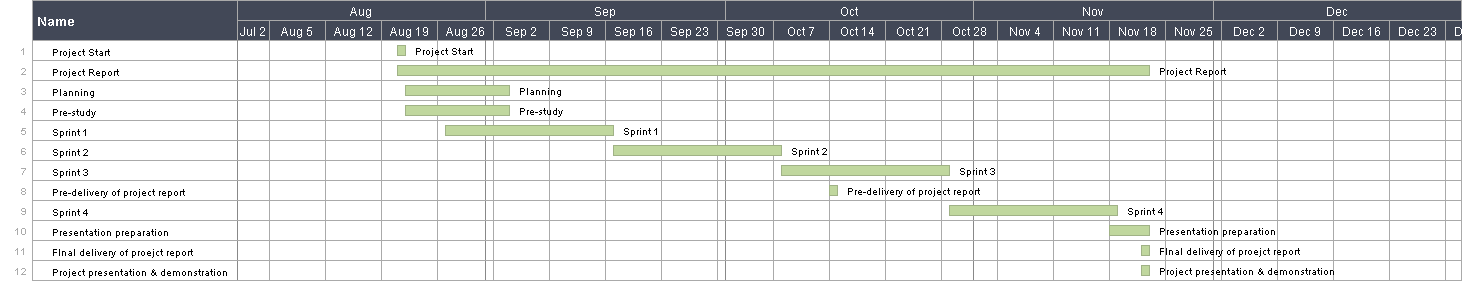
\includegraphics[width=\textwidth, height=2.5in]{foo}
\caption{Gantt-diagram for the entire project}
\end{center}
\end{figure}